\documentclass[11pt]{article}
\usepackage[margin=1in]{geometry}
\usepackage[numbers]{natbib}
\usepackage{graphicx}
\usepackage{amsmath}
\usepackage{amssymb}
\usepackage[parfill]{parskip} % new line between paragraphs, no indentation
\usepackage[colorlinks,pdfstartview=FitH,citecolor=blue, linkcolor=blue]{hyperref}
\usepackage{xcolor}
\usepackage{xeCJK} % Enabling Chinese characters
\usepackage{mdwlist} % Tight lists
\usepackage{enumerate} % Enabling options for list environments
\usepackage{float}


% Header
\usepackage{fancyhdr}
\pagestyle{fancy}
\fancyhf{}%Clear all heads and foots
\setlength{\headheight}{40pt} %Eliminate the warning of "headheight is too samll"
\rhead{Written Exam Answers\\Jianzhao Bi\\\today}
\cfoot{\thepage}

% Set font size for "section"
\usepackage{sectsty}
\sectionfont{\fontsize{11}{11}\selectfont}

% Define a new command for text subscript
\newcommand{\tsub}{\textsubscript}

\begin{document}

\section{In a single-sentence, how would you define your research question?}

\section{Missing satellite aerosol optical depth (AOD) data in Aim 1}
\begin{enumerate*}[{[a)]}]
    \item For the AOD over land surfaces, the major causes of missing data include (1) cloud cover, (2) snow/ice cover, (3) inland water bodies, and (4) no measurement (\textit{i.e.,} data points outside the satellite scanning range). These sources led to different proportions of missing data. Take New York State in 2015 as an example, the cloud-cover, snow-cover, no measurement, and inland water led to $\sim$75\%, $\sim$6\% (it increased to $\sim$20\% in the snow season), $\sim$10\%, and $< 1\%$ of missing AOD data, respectively. 
    
    The AOD observation could not be conducted in desert and semidesert regions by the original aerosol retrieval algorithm -- Dark Target (DT) \citep{kaufman1997modis, levy2007second}, because it was difficult to separate the aerosol signal from the top-of-atmosphere (TOA) reflectances at red and near-infrared wavelengths \citep{hsu2013enhanced}. Currently, a new algorithm -- Deep Blue (DB) \citep{hsu2004aerosol} utilizes blue wavelength where the surface reflectnace over land is much lower than for longer wavelength channels (\textit{i.e.,} red and near-infrared wavelengths). DB has successfully produced aerosol products over desert and semidesert areas and expanded the AOD availability to all cloud-free and snow/water-free land surfaces \citep{hsu2013enhanced}. 
    
    Major strategies dealing with the issue of missing AOD data can be classified as four categories. The first strategy is to adjust and improve current aerosol retrieval algorithms to increase available AOD estimations \citep{van2011satellite}. The second one is to utilize the spatiotemporal autocorrelation of AOD/PM\tsub{2.5} to interpolate the missing data by geostatistical interpolation approaches (\textit{e.g.,} universal kriging) \citep{kloog2011assessing, kloog2012incorporating}. The third one is using simulated AOD by chemical transport models in the regions without AOD measurements \citep{hu2017estimating}. The fourth one is to regress the missing AOD by statistical/machine learning models with AOD-related physical and land-use parameters (\textit{e.g.,} cloud fraction, meteorological parameters, elevation, \textit{etc.}) \citep{xiao2017full}.
    
    \item In my opinion, the biggest concern comes from the non-random nature of the missingness. It has been found that cloud and snow can lead to the change of AOD levels because of the shifted AOD physical characteristics under different meteorological conditions \citep{alam2014variability, kang2015correlation, emili2011high}. Thus, it may induce potential biases when missing AOD data are estimated only from existing AOD observations or under an incomplete consideration of the associations between cloud/snow and AOD. Considering the 90\% of missingness, this large proportion of potentially biased estimations might then affect the precision of PM\tsub{2.5} prediction in terms of its values and spatiotemporal patterns. For the health analyses, the measurement error of PM\tsub{2.5} can then lead to bias toward the null in estimated associations between PM\tsub{2.5} and its health outcomes \citep{sarnat2015fine}, that is, the underestimation of the adverse health effect of PM\tsub{2.5}.
    
    \item In this study, we are trying to reduce the systematic bias caused by the non-random missingness by incorporating AOD-related cloud/snow parameters in an appropriate statistical or machine learning model. For one thing, according to the validation of gap-filled AOD by the preciser ground-based AOD observations (\textit{i.e.,} AERONET data), utilizing the parameters relating to the cloud-/snow-AOD interactions (\textit{e.g.,} cloud/snow fractions) has been proven to be an effective way to estimate the systematic change of AOD levels and increase the precision of AOD estimation \citep{xiao2017full}. For another, an appropriate regression model is also key to an accurate gap-filling since the relationships between AOD and meteorological parameters are complex. The preliminary analysis of this study has shown that machine learning models (\textit{e.g.,} Random Forests and Neural Networks) performed much better than the multiple imputation model \citep{xiao2017full} which is a latest statistical model used in AOD gap-filling. This comparison indicates the advantage and potential of machine learning models dealing with complex interactions which can hardly be described by current statistical models. Admittedly, our current consideration about possible parameters explaining the cloud-/snow-AOD interactions is still limited and incomplete, and thus the bias will still exist in the AOD estimations. We will further examine more cloud/snow parameters and try to more precisely recover the relationships between cloud/snow and AOD.
\end{enumerate*}

\section{Low-cost sensor observations for \texorpdfstring{PM\tsub{2.5}}{PM2.5} predictions in Aim 2}
\begin{enumerate*}[{[a)]}]
    \item Yes. Based on some previous studies \citep{hu2017estimating, di2016assessing} and the preliminary results of this study, the convolutional layer of PM\tsub{2.5} measurements (applying a convolution kernel, here is an inverse distance weighting (IDW) kernel, on the input layer), as an additional predictor variable to account for spatial autocorrelation of PM\tsub{2.5}, has a larger contribution to the PM\tsub{2.5} predictions than satellite AOD data in the prediction models, and can significantly improve the model performance. Specifically, both \citet{hu2017estimating} and the preliminary analysis of this study showed that the PM\tsub{2.5} convolutional layers had the highest variable importance values in the PM\tsub{2.5} models based on the random forest algorithm. Similarly, in Equation (4) of the proposal, we are planning to produce a convolutional layer for low-cost sensor measurements which have a larger density than the regulatory stations, so it is expected to provide more detailed spatial patterns of PM\tsub{2.5} and have a significant contribution to the model performance. 
    
    \item Even though the PM\tsub{2.5} convolutional layer has greater influence and importance than satellite AOD in terms of the model performance, it cannot be said that satellite AOD is less important in the process of PM\tsub{2.5} estimation. The indicator of the model performance -- cross-validation -- can only be conducted in the areas with regulatory PM\tsub{2.5} stations, and these stations are currently unevenly distributed and only accumulated in the populated areas. Therefore, the model performance is unknown in the areas without regulatory stations, such as some rural areas and wild areas. As a result, it cannot be directly extrapolated that the PM\tsub{2.5} convolution is more important than the satellite data in these regions. In fact, since the satellite scans the land surfaces in the same way, unlike the PM\tsub{2.5} convolutional layer, it can provide a more stable data quality in both urban and rural areas. 
    
    Further, in order to assess the contribution of satellite AOD to the PM\tsub{2.5} predictions, we built a no-AOD prediction model in the preliminary analysis of this study. Figure \ref{fig:noaod} shows the spatial differences between full-model and no-AOD PM\tsub{2.5} in the snow season of 2015 (first 15 weeks). Compared to the no-AOD PM2.5, the full-model PM2.5 had changes in the spatial pattern with intensified on-road emissions. Hence, the pollution information provided by the satellite AOD can influence the PM\tsub{2.5} predictions in a discernible way. 
    
    \item If I had funds to invest in future data collection, I recommend first applying for the quality improvement of low-cost sensors, and then applying for the denser deployment of low-cost sensors, and finally applying for the development of new satellite sensors. In my opinion, this route can provide the quickest and most direct improvement for the PM\tsub{2.5} exposure assessment. Because of the smaller size and inexpensive deployment cost, the low-cost continuous monitoring instruments can potentially fill in gaps in the regulatory monitoring network to enhance the understanding of pollution hotspots \citep{gao2015distributed}. However, their large measurement errors hinder a wider application of them to assess compliance with air pollution standards \citep{hall2014integrating}. Once the low-cost sensors have reliable measurement qualities, it will be much easier to densely employ them to cover all population than the regulatory stations, and it might become the new ``regulatory'' measurements with high spatiotemporal coverage. Satellite sensors cannot provide direct obsevations of PM\tsub{2.5} so far, which limits their capability in PM\tsub{2.5} exposure assessment. However, satellite remote sensing can provide global-scale observation and are important to pollution event detection, transport and model prediction, and emission estimation \citep{hoff2009remote}, which are the unique advantages over the ground measurements. Consequently, satellite data are still valuable complements to the ground measurements, and with its evolving functions, it will play a more and more important role in the fields of environment and public health. 
\end{enumerate*}

\section{In your words, describe the specific parameter selection strategy for Equation 2}

\newpage
\begin{figure}[H]
    \centering
    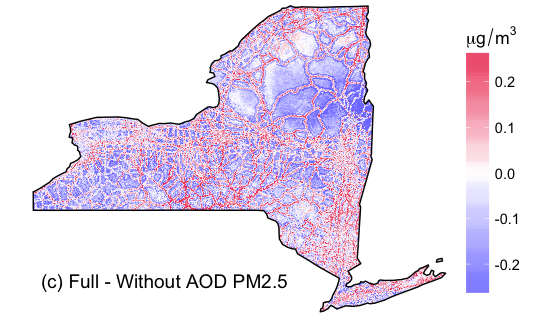
\includegraphics[width=0.7\textwidth]{img/no_aod.png}
    \caption{Spatial differences between full-model and no-AOD PM\tsub{2.5} in the snow season of 2015 (full-model minus no-AOD PM\tsub{2.5})}
    \label{fig:noaod}
\end{figure}

\newpage
\bibliographystyle{unsrtnat}
\bibliography{references}

\end{document}
